%\chapter{Wykonanie testów i dokonanie odpowiednich pomiarów}
%\section{Opis metodyki testowania}
%\section{Przebieg testów}
%\section{Analiza wyników}

\chapter{Pomiary testowe}

W celu weryfikacji poprawności działania pirometru, przeprowadzono test porównawczy z wykorzystaniem wzorcowanego pirometru przemysłowego Sonel DIT-200 wraz z opcją pomiaru temperatury metodą stykową. Test przeprowadzono w kontrolowanych warunkach laboratoryjnych w przedziale temperatury 25 - 30°C. Zakres temperatury mierzonego obiektu wynosi od 35°C do 160°C. Obiektem pomiarowym jest płyta grzejna o mocy 800W, pomalowanego na kolor czarny matowy.

\vspace{12pt}

Procedura testowa:
\begin{enumerate}
\item Przygotowanie stanowiska składającego się z urządzenia testowanego,  pirometru przemysłowego wyposażonego w pomiar metodą optyczną oraz stykową oraz obiektu odwzorowującego wymagane nastawy temperatury. \item Wykonanie pomiarów temperatury w zakresie od 35°C do 160°C w odstępach co 5°C oraz zarejestrowanie ich w arkuszu kalkulacyjnym. \item Dwukrotne powtórzenie pomiarów. Każdy pomiar był wykonywany trzykrotnie, a wyniki uśredniano w celu zwiększenia dokładności pomiarów.
\end{enumerate}

\newpage

%\section{Tabela porównawcza pomiarów}
\begin{table}[h!]
\centering
\begin{tabularx}{\textwidth}{|X|X|X|}
\hline
\textbf{Temperatura z Arduino [°C]} & \textbf{Termometr stykowy [°C]} & \textbf{Pirometr przemysłowy [°C]} \\
\hline
160 & 160 & 164.7 \\
\hline
155 & 156.1 & 159.3 \\
\hline
150 & 151.8 & 156.6 \\
\hline
145 & 146.9 & 152.9 \\
\hline
140 & 142.5 & 147.2 \\
\hline
135 & 137.2 & 142.1 \\
\hline
130 & 132.5 & 139.2 \\
\hline
125 & 127.8 & 131.3 \\
\hline
120 & 122.3 & 126.3 \\
\hline
115 & 117.4 & 120.5 \\
\hline
110 & 112.7 & 115.6 \\
\hline
105 & 106.9 & 110.7 \\
\hline
100 & 101 & 105 \\
\hline
95 & 94.8 & 100 \\
\hline
90 & 89.7 & 96.2 \\
\hline
85 & 83.8 & 92.4 \\
\hline
80 & 79.3 & 88.5 \\
\hline
75 & 73.3 & 84.1 \\
\hline
70 & 68.7 & 80.1 \\
\hline
65 & 63.8 & 75.7 \\
\hline
60 & 58.7 & 70.7 \\
\hline
55 & 54.1 & 66 \\
\hline
50 & 51 & 60.4 \\
\hline
45 & 45.4 & 54.2 \\
\hline
40 & 41.1 & 42.1 \\
\hline
35 & 37 & 36.1 \\
\hline
\end{tabularx}
\caption{Porównanie pomiarów temperatury dla różnych urządzeń.}
\label{tab:pomiary}
\end{table}
\begin{figure}[h!]
    \centering
    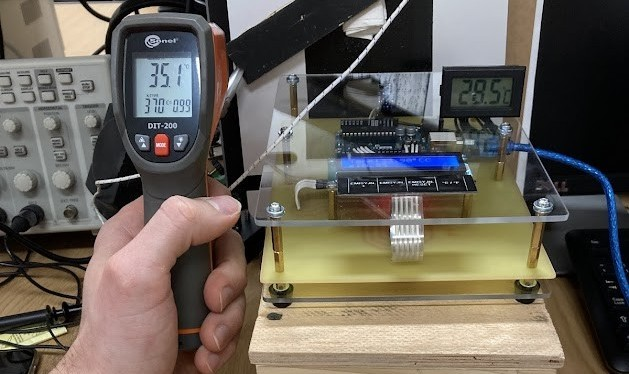
\includegraphics[width=0.6\textwidth]{images/test.jpg}
    \caption{Przebieg procedury testowej}
    \label{fig:proc}
\end{figure}